\section{Background}
\label{sec:back}

Sum-product networks (SPNs) are based on the ideas of a \emph{network polynomial}.
These are polynomial expression that encodes probability distributions.
They make use of indicator variables attached to each variable of the distribution in order to activate (indicator equals 1) or deactivate (indicator equals 0) each correspondent probability distribution variable.
When all indicators in a network polynomial are set to 1, that is they are all activated, the evaluation of the polynomial yields the unnormalized probability of the evidence.
In other words, if the probability distribution is normalized this evidence value will be 1, otherwise it will be any other real number.
The network polynomial is exponential in the number of variables, but it can be compactly represented in a graph as a SPN.

Formally, a SPN over a set of variables is a rooted directed acyclic graph with leaves being indicator variables and internal nodes being sum or products.
All edges from a sum node has non-negative weights attached to it.
The value of a product node is the product of its children and the value of a sum node is the sum of the product of the value of its children and the weights.
For example, Figure \ref{fig:spn} illustrated a SPN for a naive Bayes model presented in \citep{Poon2011}.
The SPN represents a network polynomial.
Thus, by changing the indicator variable values we set different states of the probability distribution represented by the SPN and, consequently, the network polynomial.
A SPN is then classified as a probabilistic graphical model (PGM), since it is defined by a graph with probability informations encoded.

\begin{figure}[hbt]
    \begin{center}
    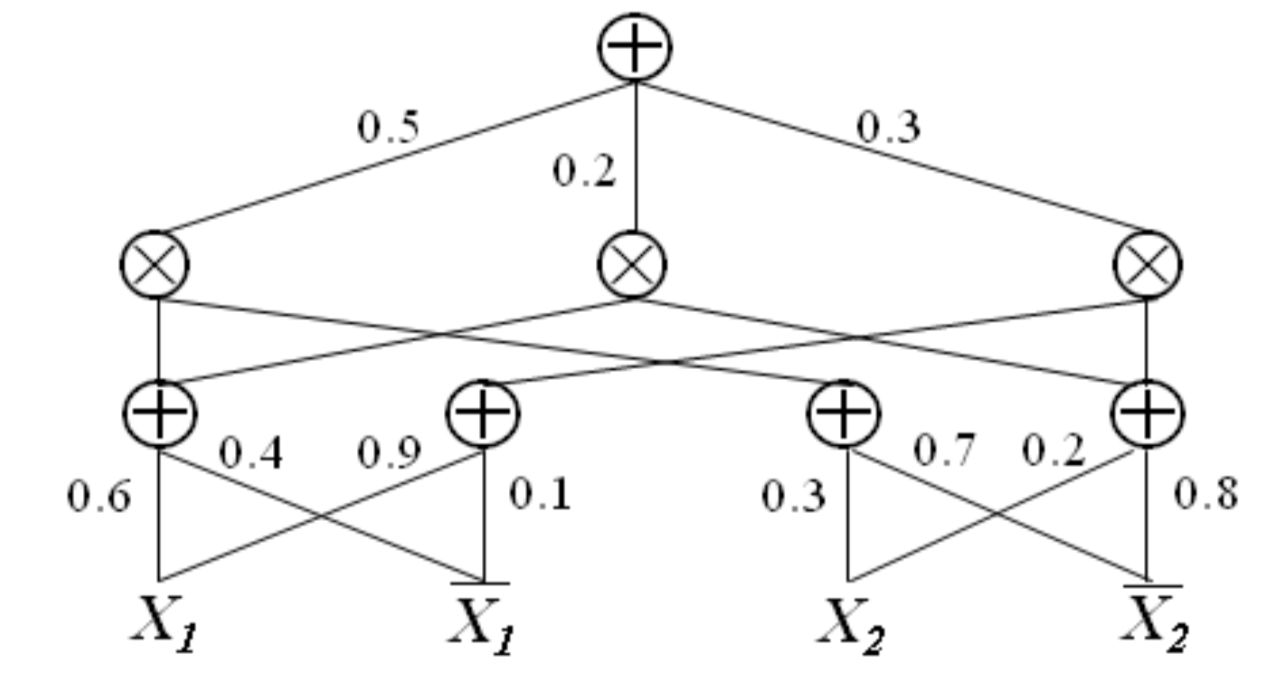
\includegraphics[width=0.6\textwidth]{figures/spn.png}
    \caption{A SPN representing a naive Bayes, as shown in \citep{Poon2011}.}
    \label{fig:spn}
    \end{center}
\end{figure}


The key advantages of SPNs are in the learning process, when compared to other PGMs.
Learning a PGM usually involves two steps: first learning the graph structure and later the probability informations.
This method is problematic when trying to optimize the learning process by limiting the size of learning informations \cite{Zhao2015}.
If a restriction is imposed on the graph size, for optimization reasons, it is not guaranteed that the probability informations will also be restricted in size.
The other way around is also true: if a restriction is applied to the size of the learned probability information, it is not guaranteed that the graph will be restricted in size.
This is a practical issue when learning PGMs.
On the other hand, SPNs has the intrinsic feature which guarantees that if the graph is restricted in size the probability information will be as well.